\documentclass[a4paper,11pt]{article}
\usepackage{amssymb}
\usepackage{amsfonts, eufrak}
\usepackage{amsmath}
\usepackage{amsthm}
\usepackage{graphicx}
\usepackage{enumerate}
\usepackage{multicol}
\usepackage[utf8x]{inputenc}

\usepackage[a4paper,top=1.2cm, bottom=1.5cm, left=1.0cm, right=1.2cm]{geometry}
\theoremstyle{definition}
\newtheorem{exe}{Questão}



\begin{document}
\renewcommand{\thefigure}{{\hspace{-.cm}{\arabic{figure}}}}
 \setcounter{figure}{0}


%\thispagestyle{empty}
\begin{center}{\sc \large MAT02280 - Estatística Básica I}\end{center}
\begin{center}{\sc Prova 1 - Turma B - 16/11/2017}\end{center}
\begin{flushright}{\sc Prof. Markus Stein}\end{flushright}

\begin{multicols}{2} 
Nome:

Cartão:

\vspace{2mm}
\begin{flushright}
\begin{tabular}{|c|c|c|c|c|c|}
  \hline
  % after \\: \hline or \cline{col1-col2} \cline{col3-col4} ...
   \hspace{6mm}1\hspace{6mm}& \hspace{6mm}2\hspace{6mm}&\hspace{6mm}3\hspace{6mm}&\hspace{6mm}4\hspace{6mm}&\hspace{6mm}5\hspace{6mm}&Total \\
   \hline
   &  &  & & &   \\
  \hline
\end{tabular}
\end{flushright}
\end{multicols}

\medskip
\medskip
\begin{exe} (2,8 pontos)
Quer se estudar o número de erros de impressão de um livro, Para isso escolheu-se uma
amostra de 50 páginas, encontrando-se o seguinte número de erros por página:

\begin{center}
 \begin{tabular}{c|c|c|c}
 \hline
 nº de erros por página & $F_j$ & $F_j \times x_j$ & $F_j \times (x_j - \bar{x})^2$ \\
 \hline
 0 &    &    & \\
 1 & 20 & 20 & 2,31\\
 2 & 3  & 6  & 5,39\\
 3 & 1  & 3  & 5,48\\
 4 & 1  & 4  & 11,16\\
 \hline
 $\sum$ &  &  & \\
 \hline
 \end{tabular}
\end{center}
(Obs: $F_j$ denota a frequência absoluta e $x_j$ o número de erros por página, na linha $j$ da tabela).

\begin{enumerate}[(a)]
  \item Qual a variável em questão? Classifique-a. Qual a unidade de observação? \\
  \item Qual o percentual de páginas com dois erros. \\
  \item E qual a porcentagem de páginas com menos de três erros? \\
  \item Indique a porcentagem de páginas com mais de três erros. \\
  \item Qual o número médio de erros por página $\bar{x}$? E número mediano $M_d$? \\
  \item Qual o desvio padrão do número de erros por página $s$? E o coeficiente de variação $CV$? \\
  \item Se o livro tem 500 páginas, qual o número de erros esperados no livro? \\
\end{enumerate}
\end{exe}

\medskip
\begin{exe} (1,8 pontos) 
Responda verdadeiro (V) ou falso (F):
\begin{enumerate}[(a) (\quad)]
  \item Metade dos valores de uma variável quantitativa são sempre menores que a média. %F
  \item Quando a variável quantitativa tem distribuição unimodal e simétrica, metade de seus valores é menor que a média. %V
  \item A média não é uma boa medida de tendência central para uma variável quantitativa com distribuição unimodal muito assimétrica, pois esta medida é muito influenciada por valores extremos. %V
  \item A mediana é quem melhor representa um conjunto de dados, pois ela é a única medida de tendência central que leva em consideração todas as observações existentes.  %F
  \item Se a média e a mediana de um conjunto de dados forem respectivamente 10 e 15 pode-se dizer que essa distribuição apresenta assimetria. %V
  \item Quanto maior a média, maior é a variância. %F
  \item Quanto maior é a variância, maior é o desvio padrão. %V
  \item O coeficiente de variação pode ser negativo. %V
\end{enumerate}
\end{exe}

\medskip
\begin{exe}(1,8 pontos)
Realizou-se uma pesquisa com o intuito de verificar o assunto de interesse dos adultos de uma certa população. Cada respondente indicou um escore de -100 a 100 referente à sua preferência para cada assunto. Os dados obtidos estão resumidos no gráfico abaixo. 
\begin{figure}[h!]
  \centering
  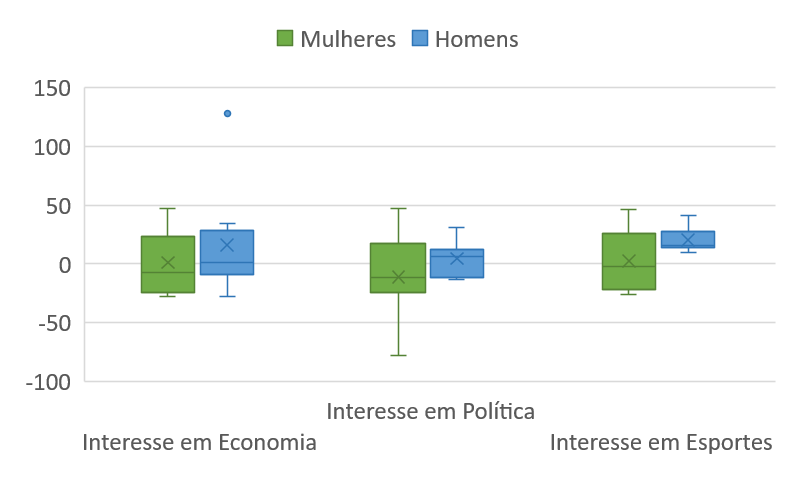
\includegraphics[width=0.6\linewidth]{boxplot_prova_2017_2.png} 
  \caption{Boxplot das preferências por sexo.}
  \label{Fig1}
\end{figure}
(Obs.: o símbolo $\times$ dentro das caixas indica a média.).
Responda:
\begin{enumerate}[(a)]
  \item Quais as variáveis analisadas? Classifique-as. \\
  % \item Interprete o gŕfico acima.
  \item Utilizando os gráficos de boxplot da figura 1 responda verdadeiro (V) 
  ou falso (F):
  \begin{enumerate}[(\quad)]
    \item Os respondentes do sexo feminino tiveram preferências semelhantes 
    entre economia e esportes.
    \item No assunto economia, as medianas enre homens e mulheres 
    são equivalentes.
    \item Os homens tenderam a informar um escore de interesse maior do que as 
    mulheres em todos os assuntos.
    \item Os escores no assunto política apresentam distribuições simétricas.
    \item No assunto esporte os escores os escores dos homens são mais homogêneos 
    do que os escores das mulheres.
  \end{enumerate}
\end{enumerate}
\end{exe}

\medskip
\begin{exe} (1,6 pontos) Responda verdadeiro (V) se a variável aleatória presente nos problemas de probabilidade abaixo possui distribuição binomial ou falso (F) caso contrário:
\begin{enumerate}[1. (\qquad)]
% \item O show 60 minutes do canal de televisão CBS tem sido um programa de sucesso por muitos anos.
% Esse show tinha uma audiência de 20, significando que dentro os aparelhos de TV ligados $20\%$ estavam
% sintonizados no 60 Minutes. Suponha que o anunciante deseja verificar se realmente o valor da audiência
% é de $20\%$ realizando a sua própria pesquisa;
\item A companhia financeira A prepara restituições de impostos para pessoas físicas. De acordo com o serviço
da Receita Federal, indivíduos que ganham entre 20.000 e 30.000 reais passam por auditoria a uma taxa
de $30\%$. A empresa quer saber a probabilidade de 5 indivíduoss em um grupo de 10 pessoas, que possuem
renda de 20.000 a 30.000, passarem por auditoria.
\item Para um período recente de 100 anos, houve 93 grandes terremotos. Qual a probabilidade de o número
de terremotos em um ano ser igual à 7.
\item Calcule a probabilidade de que o número de clientes de uma livraria em um dado dia de trabalho seja
igual à 40.
\item O tempo médio para realização de determinada tarefa é de 50 minutos, calcule a probabilidade de que
algum indivíduo realize essa tarefa em menos de 30 minutos
\end{enumerate}
\end{exe}

\newpage
\medskip
\begin{exe} (2,0 pontos)
Uma pequena companhia de seguros analisou a frequência com que todos os seus 
segurados utilizaram serviços hospitalares durante um certo período. Os 
resultados são apresentados na tabela abaixo.
\begin{center}
\begin{tabular}{cccc}
\hline
  & \multicolumn{2}{c}{Sexo} & \\
\cline{2-3}
Usou serviço hospitalar & Masculino & Feminino & $\sum$ \\ \hline
Sim     & 100 & 150 & 250   \\
Não    & 900 & 850 & 1750  \\ \hline
$\sum$  & 1000 & 1000& 2000  \\ \hline
\end{tabular}
\end{center}
Selecionando-se um segurado ao acaso, responda (utilizando o conceito de 
probabilidade frequentista):
\begin{enumerate}
  \item Qual a probabilidade de ser uma mulher e que não tenha utilizado serviços hospitalares? \\
  \item Qual a probabilidade de ser homem ou tenha utilizado serviços hospitalares? \\
	\item Sabendo que o segurado é mulher, qual a probabilidade de este ter usado serviços hospitalares? \\
  \item Qual a probabilidade de ser mulher dado que o segurado não usou serviços hospitalares? \\
\end{enumerate}
\end{exe}

\bigskip
\begin{center}{\sc Formulário}\end{center}
\begin{enumerate}
	\item {\bf Média simples}. $\bar{x} = \frac{\sum_{i=1}^n x_i}{n} $; {\bf Média ponderada}. $\bar{x} = \frac{\sum_{i=1}^n x_i \times p_i}{n} $.
	\item {\bf Mediana}. Obtenha a posição $p = \frac{n+1}{2}$, então $\mbox{Md} = x_{(p)}$.
	\item {\bf Variância}. $s^2 = \frac{\sum_{i=1}^n (x_i - \bar{x})^2}{n-1} $; {\bf Variância ponderada}. $s^2 = \frac{\sum_{i=1}^n p_i \times (x_i - \bar{x})^2}{n-1} $ 
	\item {\bf Desvio padrão}. $s = \sqrt{s^2}$
	\item {\bf Coeficiente de variação}. $\mbox{CV} = \frac{s}{\bar{x}}$
	\item {\bf Distribuição Binomial}. Probabilidade de observar $k$ `sucessos' em $n$ repetições de um ensaio de Bernoulli, onde a probabilidade de `sucesso' em cada ensaio é igual a $\pi$: $$\mathrm{Pr}[X = k] = \frac{n!}{k!(n-k)!} \pi^k(1-\pi)^{n-k} $$
\end{enumerate}

\end{document}
